% 
%  DiscussionChapter.tex
%  ThesisISEL
%  
%  Created by Sana on 2023/08/09.
%

\chapter{Discussion}
\label{cha:Discussion_chapter}

This chapter is dedicated to discuss the results and comparing them to other related works in the field.


\section{Comparison with other works} % (fold)
\label{sec:Comparison_with_other_works}

This section consists of comparisons with similar works in the field to provide a perspective from which observations and measurements are made for the evaluation of this work. Obviously, there are fundamental differences in each approach, and direct comparison cannot be drawn between the outcomes. 

The Approaches are compared under the following aspects:
\begin{itemize}
\item \textbf{Scope and applicability}: Has the model been trained on a single project and can it only classify files within that application, or is it generally applicable to any code from a large variety of sources.
\item \textbf{Programing language}: what programing language was subject of the study
\item \textbf{Machine Learning Approach}: what machine learning approach was used
\item \textbf{Vulnerability types}: which kinds of vulnerabilities can be detected.
\end{itemize}

\subsection{Discovering vulnerabilities using data-flow analysis and machine learning} % (fold)
\label{sub:related_work1}

This is the main work related to our problem. It combines static code analysis with machine learning for detecting SQL injection (SQLi) and Cross-Site Scripting (XSS) vulnerabilities in PHP applications. It also uses SAMATE for collecting training data for the model \cite{Kronjee2018}.

The work attempted to contribute and demonstrate that it is possible to combine machine learning with static code analysis for detecting vulnerabilities in software. However, we argue that the demonstrated results appear inconsistent, especially when testing the tool with different data (data from other applications). This is due to the lack of demonstration of the data extracted from other applications (The work was unable to showcase the data extracted from other applications and used for testing their tool). Furthermore, according to our analyses, we argue that the process used for feature extraction and dataset creation relies on a method that does not establish fixed features for any project (Java source code) in general. The features extracted from the source codes are the functions (function names), which can differ from project to project. In this sense, the work cannot be considered conclusive because it would not be possible to use the model created and trained with the SAMATE dataset for any other dataset extracted from a different project or source code.

We have made comparisons regarding the accuracy of their model with ours for several classifiers using SAMATE data. The following figures illustrate the results obtained for both works.

\newpage

\begin{figure}[ht]	
	\centering
	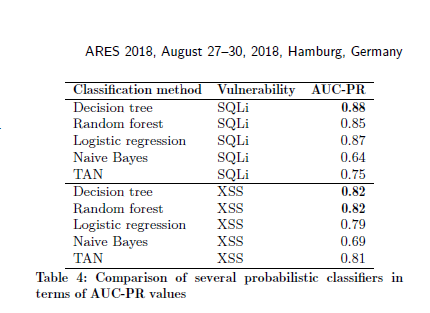
\includegraphics[width=0.90\textwidth]{Result_WIRECAML.}
	  \caption{Model evaluation result obtained by the WIRECAML tool.}
  \label{fig:bibtex}
\end{figure}

For the same classifiers, our model achieved better results compared to their model. Their work is limited in extracting features for dataset construction, and this is the main advantage of our work compared to theirs. The model created by our tool can be used for any dataset extracted from other applications since it takes into account the same features.



% subsection related_work1(end)

\subsection{VUDENC - Vulnerability Detection with Deep Learning on a Natural Codebase} % (fold)
\label{sub:related_work_vudenc}

It is a vulnerability detection system that utilizes neural networks to learn vulnerable features from a collection of data extracted from GitHub. The work focuses on the Python programming language and exclusively learns source code \cite{Wartschinski2019}. 

This work managed to demonstrate the potential use of deep learning directly on source code to learn vulnerable features, utilizing LSTM (Long Short-term Memory) models \cite{article_LSTM}.

They created the model using LSTM and managed to achieve good results. With an F1 score of around 87\%, they attained a precision of 91\% and a recall of 83\%.

Their tool was able to detect several types of vulnerabilities, and this is the main advantage of their work compared to ours. Another advantage in comparison with our approach is that they used real GitHub data for model creation. In our case, we used SAMATE data for training and model creation.



% subsection related_work_vudenc(end)

\subsection{VulDeePecker Deep Learning Based System For Vulnerability Detection} % (fold)
\label{sub:related_work_VulDeePeckerADeep}

Li et al. \cite{Zhen_Li2018} developed this tool  to detect buffer error vulnerabilities and resource management error vulnerabilities in C/C++ programs. They work on a "code gadget database" made from a large number of popular open source projects, including the Linux kernel and Firefox. The vulnerabilities are found by using the NVD and SAMATE dataset, which contain synthetic and real-life / production code, flaws, and vulnerabilities.

Selecting their data from those sources, Li et al work on very high-quality code. Just like us , they use code changes or patches to find vulnerabilities and create their own labels, but also they include a second step of human supervision to double-check every positive label manually (in contrast, the approach taken in our tool is completely automatic).


They train a bidirectional LSTM and achieve an impressive F1 score of around 85-95\%. Our tool achieve quite the same high score too. Furthermore, the their database only consists of synthetic code as well.

The authors of VulDeePecker compare their tool to other approaches and find an F1 score of 27\% for the tool Flawfinder, 47\% for Checkmarx, and 18.2\% for VulPecker. The latter two, however, are optimized to have close to zero false positives, which was not accomplished in our case.

% subsection related_work_VulDeePeckerADeep(end)

% section Comparison_with_other_works (end)

\section{Limitations} % (fold)
\label{sec:LIMITATIONS_SEC}

The present design, implementation, and evaluation of this work have several limitations, which suggest interesting open problems for future research.  First, the present design of this work is limited to deal with a variety of different types of vulnerabilities. The feature extraction process is very challenging prolem for projects compatibilities with Java programming language version 8, as well as with higher versions due to the functional programming paradigms (dealing with lambda expressions on faetures extraction).

Second, the present design of our tool only deals with Java programs. Future research needs to be conducted to adapt it to deal with other kinds of programming languages.

Third, the present design of this work only deals with vulnerabilities related to functions invocation. The future work could investigate how to detect the other kinds of vulnerabilities by leveraging the other kinds of key points.

Fourth, The data collected for model creation was just from one source (SAMATE) and  insufficient, it's necessary to collect more data from different sources and from real example source code.

Fifth, the model evaluation process using standard performance measures for the classifier that have been applied in other works regarding vulnerability prediction, threats to conclusion validity are minimized.  We used  predictions, accuracy, precision, and recall metrics to evaluate the performance of the model. However, in practice, there may be other metrics and representation demonstrating how well a classifier performs.

Sixth, the present implementation of our tool is limited to the machine learning classifier. We can conduct systematic experiments with other kinds of 
unsupervised learning that could be used for vulnerability detection.

Seventh, the present  method of model creation is limited because the Hyperparameter tuning process was not used. It can be a crucial step in model creation to tune parameters in machine learning in order to adjusting the settings of a machine learning algorithm or model to ensure that the model performs at its best.

Finally,  Furthermore, design decisions were made which might affect the overall end result.


% section LIMITATIONS_SEC (end)

\section{Future work} % (fold)
\label{sec:Future_work}

There are several unsolved issues for future research in this field of study. Firstly, the approach itself could probably be adjusted and improved, for instance, by optimizing the feature extraction process or more data collection as discussed earlier. 

The 'Var' attribute values could be refine in order to match exactly the same pattern with the truly vulnerable codes In order to improve false positives cases from the model.

Our data set is very biased due to the fact that each source code line is a sample and there are obviously many more non-vulnerable lines than vulnerable ones. The data could be compiled and filtered more thoroughly, leading to much more representative samples. By colllecting more data from different source, it could be ensured that a larger percentage of the samples actually contains more relevant examples.

Consequently, even some vulnerables scenarios that could not be taken into account in this work due to low quality data could receive the attention they deserve. Given that, the data for choosing the best parameters for the models had to be with training data because the approach did not yield enough examples, or too many unrelated results, improving the process of gathering data is highly promising. It seems plausible that an underlying dataset of higher quality would be the main contributor to a better end result.

Experiments using code in different programing language are of interest. The proposed approach could be extended to other programming languages such as PHP, C++ or C\#.
A first step would be to check if the feature extraction process (data transformation) for those programming languages can be created with the same success. Then, the model could be trained on vulnerability datasets in those other languages and compared to the works of other researchers.
The proposed approach could also be applied to specific other types of applications including a specific focus on web applications, mobile applications or software in specific domains that come with their own typical security risks.

The approach could also be extended to alert defects and bugs of other kinds in code. There is a whole research area dealing with this problem, and the application of machine learning can surely offer valuable insights. The possibilities are vast, and a lot of work is still to be done in this area.

Finally, a subsequent expansion could involve building a fully functional vulnerability detection system with high usability that takes code as input and detect vulnerabilities. While a simple prototype has already been constructed in this work, it has not been optimized for usability in daily programming. One option would be to create a plugin for an IDE or a highly customized command line tool.

% section Future_work (end)